% ------------------------------------------------------------------------------
% TYPO3 CMS 7.0 - What's New (English Version)
%
% @author	Michael Schams <schams.net>
% @license	Creative Commons BY-NC-SA 3.0
% @link		http://typo3.org/download/release-notes/whats-new/
% @language	English
% ------------------------------------------------------------------------------

% change the default aspect ratio and frame size
% \documentclass[aspectratio=43]{beamer}
%
% specify vertical top alignment globally by the [t] class option:
% \documentclass[t]{beamer}
%
% for single frames, use the same option locally:
% \begin{frame}[t] ... \end{frame}

\documentclass[t]{beamer}

% suppress navigation bar
\beamertemplatenavigationsymbolsempty

\mode<presentation>
{
	\usetheme{typo3slides}
}

% global variables
\title{TYPO3 CMS 7.0 - What's New}
\subtitle{Summary of the new features, changes and improvements}
\author{
	\centerline{Created by:}
	\centerline{Patrick Lobacher and Michael Schams}
}

\date{\today}

\begin{document}

% select TYPO3 Share font
\sharefont

% ------------------------------------------------------------------------------
% LTXE-CHAPTER-TITLEPAGE
% ------------------------------------------------------------------------------

\begingroup
	\setbeamercolor{normal text}{fg=white,bg=typo3orange}
	\setbeamercolor{title}{fg=white}
	\setbeamercolor{author}{fg=white}
	\setbeamertemplate{footline}[default]
	\begin{frame}
		\titlepage
	\end{frame}
\endgroup

% ------------------------------------------------------------------------------
% LTXE-CHAPTER-TABLEOFCONTENTS
% ------------------------------------------------------------------------------

% between two frames: use \newpage (not \clearpage!) to force a column break:
% \addtocontents{toc}{\newpage}

\section*{TYPO3 CMS 7.0 - What's New}
\begin{frame}[fragile]
	\frametitle{Chapter Overview}
	\framesubtitle{Chapter Overview}

	\begin{multicols}{2}
		\tableofcontents
	\end{multicols}

\end{frame}

% ------------------------------------------------------------------------------
% LTXE-CHAPTERS-START
% Chapter: Introduction
% ------------------------------------------------------------------------------

% ------------------------------------------------------------------------------
% TYPO3 CMS 7.2 - What's New - Chapter "Introduction" (English Version)
%
% @author	Michael Schams <schams.net>
% @license	Creative Commons BY-NC-SA 3.0
% @link		http://typo3.org/download/release-notes/whats-new/
% @language	English
% ------------------------------------------------------------------------------
% LTXE-CHAPTER-UID:		16517900-07a67f43-fe9f3e35-7e924788
% LTXE-CHAPTER-NAME:	Introduction
% ------------------------------------------------------------------------------

\section{Uvod}
\begin{frame}[fragile]
	\frametitle{Uvod}

	\begin{center}\huge{Uvod}\end{center}
	\begin{center}\huge{\color{typo3darkgrey}\textbf{Cinjenice}}\end{center}

\end{frame}

% ------------------------------------------------------------------------------
% LTXE-SLIDE-START
% LTXE-SLIDE-UID:		dce36242-c42d3b1a-9256338c-7ba3f3b9
% LTXE-SLIDE-ORIGIN:	6d5e9f3e-f9d9677e-43d7d497-e80ba9ef English
% LTXE-SLIDE-TITLE:		TYPO3 CMS 7.2 - The Facts
% ------------------------------------------------------------------------------
\begin{frame}[fragile]
	\frametitle{Uvod}
	\framesubtitle{TYPO3 CMS 7.2 - Cinjenice}

	\begin{itemize}
		\item Datum objavljivanja: 28. april 2015.
		\item Tip objavljivanja: "Brza objava" ("Sprint Release")
		\item Vizija: Prihvatiti, inovirati, dostaviti
		\item Glavni fokus: Korisnicki interfejs
	\end{itemize}

	\begin{figure}
		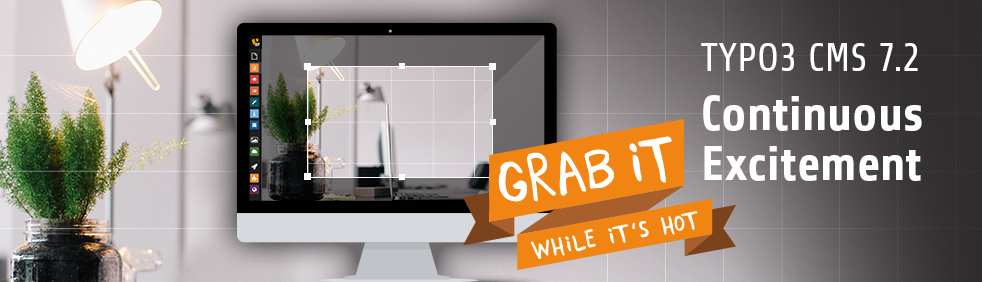
\includegraphics[width=0.95\linewidth]{Introduction/typo3cms72-teaser.png}
	\end{figure}

\end{frame}

% ------------------------------------------------------------------------------
% LTXE-SLIDE-START
% LTXE-SLIDE-UID:		be262c6f-e46fb037-7681e9f5-b16ddef1
% LTXE-SLIDE-ORIGIN:	759c3860-d5061f6e-2bb0009f-6ea130c8 English
% LTXE-SLIDE-TITLE:		System Requirements
% ------------------------------------------------------------------------------
\begin{frame}[fragile]
	\frametitle{Uvod}
	\framesubtitle{Sistemski zahtevi}

	\begin{itemize}
		\item PHP*:\tabto{3cm}v5.5.0 - v5.6.x
		\item MySQL:\tabto{3cm}v5.5.x - v5.6.x (no strict mode)
		\item Prostor na disku:\tabto{3cm}min 200 MB
		\item PHP podesavanja:

			\begin{itemize}
				\item memory\_limit >= 128M
				\item max\_execution\_time >= 240s
				\item opcija \texttt{--disable-ipv6} \underline{ne sme} se koristit
			\end{itemize}

		\item Administratorski interfejs zahteva IE >= 9 ili bilo koji drugi moderni pretrazivac

	\end{itemize}

	\vspace{1cm}
	*) Dodatno objasnjenje: \href{http://typo3.org/news/article/php-minimum-requirements-for-typo3-cms-7/}{PHP Minimum Requirements for TYPO3 CMS 7}

\end{frame}

% ------------------------------------------------------------------------------
% LTXE-SLIDE-START
% LTXE-SLIDE-UID:		a591867d-d1b6280a-b6f4d9e7-c592c674
% LTXE-SLIDE-ORIGIN:	70c77c41-e2b83d82-2f182996-98061070 English
% LTXE-SLIDE-TITLE:		Development And Release Timeline
% ------------------------------------------------------------------------------
\begin{frame}[fragile]
	\frametitle{Uvod}
	\framesubtitle{Vreme razvoja i datumi objavljivanja}

	\begin{figure}
		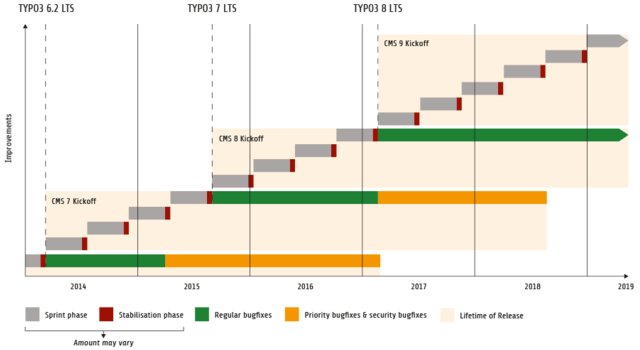
\includegraphics[width=0.90\linewidth]{Introduction/ReleaseAgenda.png}
	\end{figure}

\end{frame}

% ------------------------------------------------------------------------------
% LTXE-SLIDE-START
% LTXE-SLIDE-UID:		650837ac-b27fb921-fe403d6d-4d8c8a81
% LTXE-SLIDE-ORIGIN:	b55d3fe9-76807061-d97f3fee-7db1f190 English
% LTXE-SLIDE-TITLE:		TYPO3 CMS Roadmap
% ------------------------------------------------------------------------------
\begin{frame}[fragile]
	\frametitle{Uvod}
	\framesubtitle{TYPO3 CMS plan}

	Predvidjeni datumi objavljivanja i njihov osnovni fokus:

	\begin{itemize}
		\item v7.0 \tabto{1.0cm}02/Dec/2014\tabto{3.4cm}Remont administratorskog interfejsa prvi deo
		\item v7.1 \tabto{1.0cm}24/Feb/2015\tabto{3.4cm}Ciscenje osnove sistema i optimizacija

		\item
			\begingroup
				\color{typo3orange}
					v7.2 \tabto{1.0cm}28/Apr/2015\tabto{3.4cm}Korisnicki interfejs
			\endgroup

		\item v7.3 \tabto{1.0cm}09/Jun/2015\tabto{3.4cm}Ekosistem za dodatke, Composer\newline
			\tabto{3.4cm}i upravljanje prosirenjima
		\item v7.4 \tabto{1.0cm}04/Aug/2015\tabto{3.4cm}Remont administratorskog interfejsa drugi deo
		\item v7.5 \tabto{1.0cm}29/Sep/2015\tabto{3.4cm}\textit{(bice odredjeno...)}
		\item v7.6 \tabto{1.0cm}xx/xxx/2015\tabto{3.4cm}\textbf{TYPO3 CMS 7 LTS}\newline
			\tabto{3.4cm}(Verzija sa dugorocnom podrskom)
	\end{itemize}

	\smaller
		\url{https://typo3.org/typo3-cms/roadmap/}\newline
		\url{http://typo3.org/news/article/embrace-and-innovate-typo3-cms-7/}
	\normalsize

\end{frame}

% ------------------------------------------------------------------------------
% LTXE-SLIDE-START
% LTXE-SLIDE-UID:		120f3d6f-b2ee06ee-7729b0e0-32a6a99a
% LTXE-SLIDE-ORIGIN:	b0c28f26-c3ca2e99-195954a8-ed76f9d4 English
% LTXE-SLIDE-TITLE:		Installation
% ------------------------------------------------------------------------------
\begin{frame}[fragile]
	\frametitle{Uvod}
	\framesubtitle{Instalacija}

	\begin{itemize}
		\item Zvanicna procedura za instalaciju na Linux/Mac OS X\newline
			(DocumentRoot na primer \texttt{/var/www/site/htdocs}):
		\begin{lstlisting}
			$ cd /var/www/site
			$ wget --content-disposition get.typo3.org/7.2
			$ tar xzf typo3_src-7.2.0.tar.gz
			$ cd htdocs
			$ ln -s ../typo3_src-7.2.0 typo3_src
			$ ln -s typo3_src/index.php
			$ ln -s typo3_src/typo3
			$ touch FIRST_INSTALL
		\end{lstlisting}

		\item Simbolicki linkovi (Symbolic links) na Microsoft Windows:

			\begin{itemize}
				\item Koristiti \texttt{junction} za Windows XP/2000
				\item Koristiti \texttt{mlink} za Windows Vista i Windows 7
			\end{itemize}

	\end{itemize}
\end{frame}

% ------------------------------------------------------------------------------
% LTXE-SLIDE-START
% LTXE-SLIDE-UID:		7fe5ca06-5b7485e7-1d868a10-d1e84aa4
% LTXE-SLIDE-ORIGIN:	48136734-ae508d23-bce5811d-667f8908 English
% LTXE-SLIDE-TITLE:		Upgrade to TYPO3 CMS 7
% ------------------------------------------------------------------------------
\begin{frame}[fragile]
	\frametitle{Uvod}
	\framesubtitle{Nadogradnja na TYPO3 CMS 7.x}

	\begin{itemize}
		\item Nadogradnja je moguca samo sa TYPO3 CMS 6.2 LTS
		\item TYPO3 CMS < 6.2 bi prvo trebalo nadograditi na TYPO3 CMS 6.2 LTS
	\end{itemize}

	\begin{itemize}

		\item Upsutstvo za nadogradnju:\newline
			\smaller\url{http://wiki.typo3.org/Upgrade#Upgrading_to_7.2}\normalsize
		\item Zvanicni TYPO3 vodic "TYPO3 Installation and Upgrading":
			\smaller\url{http://docs.typo3.org/typo3cms/InstallationGuide}\normalsize
		\item Opsti pristup:
			\begin{itemize}
				\item Proveriti minimalne sistemske zahte \small(PHP, MySQL, itd.)
				\item Proveriti \textbf{deprecation\_*.log} u staroj TYPO3 instanci
				\item Nadograditi sva prosirenja na najnoviju verziju
				\item Postaviti nove fajlove i pokrenuti Install Tool \textrightarrow Upgrade Wizard
				\item Proveriti startup modul za administratore (opciono)
			\end{itemize}
	\end{itemize}

\end{frame}

% ------------------------------------------------------------------------------


% ------------------------------------------------------------------------------
% Chapter 1: Backend User Interface
% ------------------------------------------------------------------------------

% ------------------------------------------------------------------------------
% TYPO3 CMS 7.3 - What's New (German Version)
%
% @author	Patrick Lobacher <patrick@lobacher.de> and Michael Schams <schams.net>
% @license	Creative Commons BY-NC-SA 3.0
% @link		http://typo3.org/download/release-notes/whats-new/
% @language	German
% ------------------------------------------------------------------------------
% LTXE-CHAPTER-UID:		cc6b358d-f0ed36d3-f7a72fa2-af63ccfc
% LTXE-CHAPTER-NAME:	Backend User Interface
% ------------------------------------------------------------------------------

\section{Backend User Interface}
\begin{frame}[fragile]
	\frametitle{Backend User Interface}

	\begin{center}\huge{Kapitel 1:}\end{center}
	\begin{center}\huge{\color{typo3darkgrey}\textbf{Backend User Interface}}\end{center}

\end{frame}

% ------------------------------------------------------------------------------
% LTXE-SLIDE-START
% LTXE-SLIDE-UID:		b4dc1576-57b4854f-26a32d85-11f7c52b
% LTXE-SLIDE-TITLE:		Feature #66173: Allow page title edit by doubleclick
% LTXE-SLIDE-REFERENCE:	Feature-66173-AllowPageTitleEditByDoubleclick.rst
% ------------------------------------------------------------------------------
\begin{frame}[fragile]
	\frametitle{Backend User Interface}
	\framesubtitle{Seitentitel im Page- und List-Modul}

	Im Page- und List-Modul kann man den Seitentitel entweder per Doppelklick
	oder mit Klick auf das Bearbeitungssymbol ändern.

	\begin{figure}
		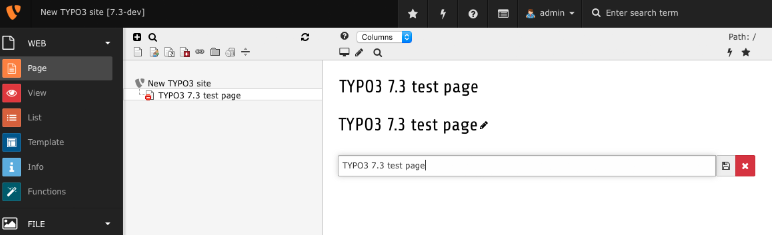
\includegraphics[width=0.9\linewidth]{BackendUserInterface/66173.png}
	\end{figure}

\end{frame}

% ------------------------------------------------------------------------------
% LTXE-SLIDE-START
% LTXE-SLIDE-UID:		168b1424-1ebb2552-ed5bac3e-8a9ac737
% LTXE-SLIDE-TITLE:		Feature #67071: Processed files cleanup tool added in Install Tool
% LTXE-SLIDE-REFERENCE:	Feature-67071-ProcessedFilesCleanupToolAddedInInstallTool.rst
% ------------------------------------------------------------------------------
\begin{frame}[fragile]
	\frametitle{Backend User Interface}
	\framesubtitle{Prozessierte FAL Dateien im Install Tool löschen}

	Das Install Tool enthält nun ein neues Tool (unterhalb von "Clean up"), um
	prozessierte FAL Dateien (wie z.B. Thumbnails) zu löschen. Das ist
	insbesondere hilfreich, wenn man grafik-relevante Settings ändern oder wenn
	man GraphicsMagick/ImageMagick aktualisiert hat und alle Dateien neu
	generieren will.

	\begin{figure}
		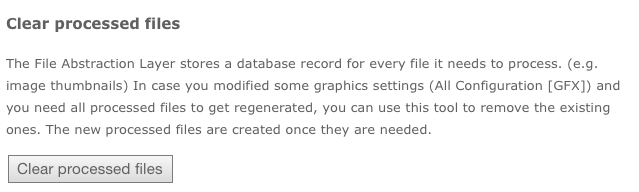
\includegraphics[width=0.6\linewidth]{BackendUserInterface/67071.png}
	\end{figure}

\end{frame}

% ------------------------------------------------------------------------------
% LTXE-SLIDE-START
% LTXE-SLIDE-UID:		daa83c1e-08d2716b-de74cbda-42361551
% LTXE-SLIDE-TITLE:		Feature #67319: Add field "copyright" to EXT:filemetadata
% LTXE-SLIDE-REFERENCE:	Feature-67319-AddFieldCopyrightToEXTfilemetadata.rst
% ------------------------------------------------------------------------------
\begin{frame}[fragile]
	\frametitle{Backend User Interface}
	\framesubtitle{Copyright in FAL Meta-Daten}

	In den zusätzlichen FAL Meta-Daten (Extension: \texttt{filemetadata}) gibt
	es nun ein Feld "\textbf{Copyright}".

	\begin{figure}
		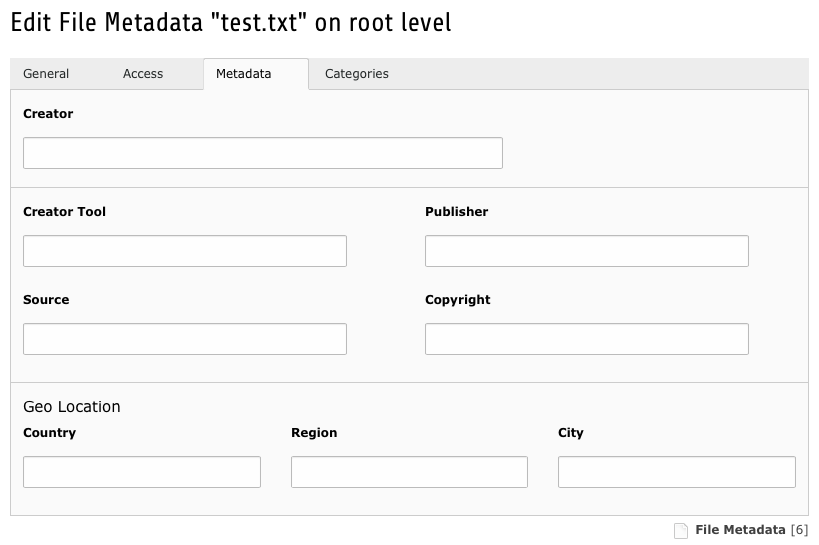
\includegraphics[width=0.6\linewidth]{BackendUserInterface/67319.png}
	\end{figure}

\end{frame}

% ------------------------------------------------------------------------------


% ------------------------------------------------------------------------------
% Chapter 2: TypoScript
% ------------------------------------------------------------------------------

% ------------------------------------------------------------------------------
% TYPO3 CMS 7.0 - What's New - Chapter "TypoScript" (German Version)
%
% @author	Patrick Lobacher <patrick@lobacher.de>
% @license	Creative Commons BY-NC-SA 3.0
% @link		http://typo3.org/download/release-notes/whats-new/
% @language	German
% ------------------------------------------------------------------------------
% LTXE-CHAPTER-UID:		d92ab5b9-9ffa4925-30a2e34f-0d6939e5
% LTXE-CHAPTER-NAME:	TypoScript
% ------------------------------------------------------------------------------
% LTXE-SLIDE-START
% LTXE-SLIDE-UID:		4bc3c9cc-59d06820-c6f719d4-6798606a
% LTXE-SLIDE-ORIGIN:	xxxxxxxx-xxxxxxxx-xxxxxxxx-xxxxxxxx
% LTXE-SLIDE-TITLE:		TSconfig Available to Link Checkers
% LTXE-SLIDE-REFERENCE:	https://forge.typo3.org/issues/54518
% ------------------------------------------------------------------------------

\begin{frame}[fragile]
	\frametitle{TSconfig \& TypoScript}
	\framesubtitle{TSconfig für Linkvalidator inkludieren}

	\begin{itemize}
		\item TSconfig Konfiguration für den Linkvalidator wird gelesen...

			\begin{itemize}
				\item entweder aus dem aktiven TSconfig des Backends,
				\item oder aus der Konfiguration des Scheduler-Tasks
			\end{itemize}

		\item Das folgende TSconfig kann vom Linkchecker ausgelesen werden

			\lstinline!mod.linkvalidator.mychecker.myvar = 1!

		\item Dort steht das TSconfig dann als \texttt{\$this->tsConfig} zur Verfügung
	\end{itemize}

\end{frame}

% ------------------------------------------------------------------------------
% LTXE-SLIDE-START
% LTXE-SLIDE-UID:		2cb2a467-28128785-d607951d-6da71df7
% LTXE-SLIDE-ORIGIN:	xxxxxxxx-xxxxxxxx-xxxxxxxx-xxxxxxxx
% LTXE-SLIDE-TITLE:		Links zu deaktivierten Datensätzen im Linkhandler melden
% LTXE-SLIDE-REFERENCE:	https://forge.typo3.org/issues/54519
% ------------------------------------------------------------------------------

\begin{frame}[fragile]
	\frametitle{TSconfig \& TypoScript}
	\framesubtitle{Links zu deaktivierten Datensätzen im Linkhandler melden}

	\begin{itemize}
		\item Bisher hat der Linkhandler lediglich gewarnt, wenn es Links zu gelöschten oder nicht existierenden Datensätzen gab
		\item Über die folgende TSconfig Einstellung kann nun auch eine Warnung aktiviert werden, wenn der Link auf einen deaktivierten Datensatz zeigt:

			\lstinline!mod.linkvalidator.linkhandler.reportHiddenRecords = 1!

	\end{itemize}

\end{frame}

% ------------------------------------------------------------------------------
% LTXE-SLIDE-START
% LTXE-SLIDE-UID:		fc40447a-69c717a6-a98ff939-1c8ed1a2
% LTXE-SLIDE-ORIGIN:	xxxxxxxx-xxxxxxxx-xxxxxxxx-xxxxxxxx
% LTXE-SLIDE-TITLE:		RTE: mehrere CSS Klassen
% LTXE-SLIDE-REFERENCE:	https://forge.typo3.org/issues/51905
% ------------------------------------------------------------------------------

\begin{frame}[fragile]
	\frametitle{TSconfig \& TypoScript}
	\framesubtitle{RTE: mehrere CSS Klassen}

	\begin{itemize}
		\item Um das Handling mit komplexen CSS Frameworks wie Twitter Bootstrap zu handhaben, muss es möglich sein, mehrere Klassen an ein Element zu vergeben
		\item Mit diesem neuen Feature muss der Autor nur noch einen Style auswählen, um dies zu erreichen, und nicht mehrere

			\begin{lstlisting}
				RTE.classes.[ *classname* ] {
				  .requires = list of CSS classes
				}
			\end{lstlisting}

	\end{itemize}

\end{frame}

% ------------------------------------------------------------------------------
% LTXE-SLIDE-START
% LTXE-SLIDE-UID:		4ba6854b-2a858198-9016aae5-39f8700d
% LTXE-SLIDE-ORIGIN:	xxxxxxxx-xxxxxxxx-xxxxxxxx-xxxxxxxx
% LTXE-SLIDE-TITLE:		RTE: nicht-selektierbare Klassen
% LTXE-SLIDE-REFERENCE:	https://forge.typo3.org/issues/58122
% ------------------------------------------------------------------------------

\begin{frame}[fragile]
	\frametitle{TSconfig \& TypoScript}
	\framesubtitle{RTE: nicht-selektierbare Klassen}

	\begin{itemize}
		\item Man kann nun Klassen als "nicht-selektierbar" im Style-Selektor des RTE konfigurieren

			\begin{lstlisting}
				// der Wert "1" bedeutet, class ist auswaehlbar
				// der Wert "0" bedeutet, class ist nicht auswaehlbar
				RTE.classes.[ *classname* ] {
				  .selectable = 1
				}
			\end{lstlisting}

	\end{itemize}

\end{frame}

% ------------------------------------------------------------------------------
% LTXE-SLIDE-START
% LTXE-SLIDE-UID:		fba34bad-dabea95b-4ed6b0af-d58e4c2e
% LTXE-SLIDE-ORIGIN:	xxxxxxxx-xxxxxxxx-xxxxxxxx-xxxxxxxx
% LTXE-SLIDE-TITLE:		RTE: mehrere CSS-Dateien einbinden
% LTXE-SLIDE-REFERENCE:	https://forge.typo3.org/issues/50039
% ------------------------------------------------------------------------------

\begin{frame}[fragile]
	\frametitle{TSconfig \& TypoScript}
	\framesubtitle{RTE: mehrere CSS-Dateien einbinden}

	\begin{itemize}
		\item Man kann nun mehrere CSS-Dateien in den RTE laden

			\begin{lstlisting}
				RTE.default.contentCSS {
				  file1 = fileadmin/rte_stylesheet1.css
				  file2 = fileadmin/rte_stylesheet2.css
				}
			\end{lstlisting}

		\item Gibt man keine CSS Datei an, so wird die Default-Datei geladen:\newline
			\texttt{typo3/sysext/rtehtmlarea/res/contentcss/default.css}
	\end{itemize}

\end{frame}

% ------------------------------------------------------------------------------
% LTXE-SLIDE-START
% LTXE-SLIDE-UID:		ae64ffca-43d35dbd-2e2eeaaf-9266d73c
% LTXE-SLIDE-ORIGIN:	xxxxxxxx-xxxxxxxx-xxxxxxxx-xxxxxxxx
% LTXE-SLIDE-TITLE:		Exception während Rendering erzeugen - Teil 1
% LTXE-SLIDE-REFERENCE:	https://forge.typo3.org/issues/47919
% ------------------------------------------------------------------------------

\begin{frame}[fragile]
	\frametitle{TSconfig \& TypoScript}
	\framesubtitle{Exception während Rendering erzeugen - Teil 1}

	\begin{itemize}
		\item Sobald Fehler im Rendering von einzelnen Inhaltselementen (Content Objects) (z.B. mittels \texttt{USER}) auftreten, wird eine Fehlermeldung erzeugt, die in TYPO3 CMS < 7.0 die gesamte Ausgabe zerstört
		\item In TYPO3 CMS 7.0 wurde ein Exception-Handling eingeführt, welches eine Fehlermeldung in die Ausgabe an der Stelle integriert, an der das Rendering stattgefunden hat
	\end{itemize}

\end{frame}

% ------------------------------------------------------------------------------
% LTXE-SLIDE-START
% LTXE-SLIDE-UID:		9eb5e70e-826968d1-b3e7c2d8-4db8fb44
% LTXE-SLIDE-ORIGIN:	xxxxxxxx-xxxxxxxx-xxxxxxxx-xxxxxxxx
% LTXE-SLIDE-TITLE:		Exception während Rendering erzeugen - Teil 2
% LTXE-SLIDE-REFERENCE:	https://forge.typo3.org/issues/47919
% ------------------------------------------------------------------------------

\begin{frame}[fragile]
	\frametitle{TSconfig \& TypoScript}
	\framesubtitle{Exception während Rendering erzeugen - Teil 2}

	\lstset{
		basicstyle=\tiny\ttfamily
	}

	\begin{lstlisting}
		# default exception handler (activated in context "production")
		config.contentObjectExceptionHandler = 1

		# configuration of a class for the exception handling
		config.contentObjectExceptionHandler =
		  TYPO3\CMS\Frontend\ContentObject\Exception\ProductionExceptionHandler

		# customised error message (show random error code)
		config.contentObjectExceptionHandler.errorMessage = Oops an error occurred. Code: %s

		# configuration of exception codes, which are not dealt with
		tt_content.login.20.exceptionHandler.ignoreCodes.10 = 1414512813

		# deactivation of exception handling for a specific plugins or content objects
		tt_content.login.20.exceptionHandler = 0

		# ignoreCodes and errorMessage can be configured globally...
		config.contentObjectExceptionHandler.errorMessage = Oops an error occurred. Code: %s
		config.contentObjectExceptionHandler.ignoreCodes.10 = 1414512813

		# ...or locally for individual content objects
		tt_content.login.20.exceptionHandler.errorMessage = Oops an error occurred. Code: %s
		tt_content.login.20.exceptionHandler.ignoreCodes.10 = 1414512813
	\end{lstlisting}

\end{frame}

% ------------------------------------------------------------------------------


% ------------------------------------------------------------------------------
% Chapter 3: In-Depth Changes
% ------------------------------------------------------------------------------

% ------------------------------------------------------------------------------
% TYPO3 CMS 7.4 - What's New - Chapter "In-Depth Changes" (English Version)
%
% @author	Michael Schams <schams.net>
% @license	Creative Commons BY-NC-SA 3.0
% @link		http://typo3.org/download/release-notes/whats-new/
% @language	English
% ------------------------------------------------------------------------------
% LTXE-CHAPTER-UID:		9a69925b-ed88557b-d362988a-940ed520
% LTXE-CHAPTER-NAME:	In-Depth Changes
% ------------------------------------------------------------------------------

\section{Korenite promene}
\begin{frame}[fragile]
	\frametitle{Korenite promene}

	\begin{center}\huge{Poglavlje 4:}\end{center}
	\begin{center}\huge{\color{typo3darkgrey}\textbf{Korenite promene}}\end{center}

\end{frame}

% ------------------------------------------------------------------------------
% LTXE-SLIDE-START
% LTXE-SLIDE-UID:		5f06bf16-98a5e8f7-05abc446-cf12e93a
% LTXE-SLIDE-ORIGIN:	5fa3f922-971c07f7-2ec96457-63394b8b English
% LTXE-SLIDE-ORIGIN:	5cfc1d44-3d6f3d87-789957ab-655f357d German
% LTXE-SLIDE-TITLE:		Breaking #65305: DriverInterface has been extended
% LTXE-SLIDE-REFERENCE:	Breaking-65305-AddFunctionsToDriverInterface.rst
% ------------------------------------------------------------------------------

\begin{frame}[fragile]
	\frametitle{Korenite promene}
	\framesubtitle{Driver Interface}

	% decrease font size for code listing
	\lstset{basicstyle=\tiny\ttfamily}

	\begin{itemize}

		\item Sledece metode pridodate su \texttt{DriverInterface}:

			\begin{itemize}
				\item \texttt{getFolderInFolder}
				\item \texttt{getFileInFolder}
			\end{itemize}

		\item Svaki FAL drajver trebalo bi da implementira ove nove metode:

			\begin{columns}[T]
				\begin{column}{.07\textwidth}
                \end{column}
				\begin{column}{.465\textwidth}

					\begin{lstlisting}
						public function getFoldersInFolder(
						  $folderIdentifier,
						  $start = 0,
						  $numberOfItems = 0,
						  $recursive = FALSE,
						  array $folderNameFilterCallbacks = array(),
						  $sort = '',
						  $sortRev = FALSE
						);
					\end{lstlisting}

                \end{column}
				\begin{column}{.465\textwidth}

					\begin{lstlisting}
						public function getFileInFolder(
						  $fileName,
						  $folderIdentifier
						);
					\end{lstlisting}

				\end{column}
			\end{columns}

	\end{itemize}

	\breakingchange

\end{frame}

% ------------------------------------------------------------------------------
% LTXE-SLIDE-START
% LTXE-SLIDE-UID:		4aba2397-08577ce4-d7092e6b-fb1739bf
% LTXE-SLIDE-ORIGIN:	603042c6-c0caed8e-a6565d08-09528be6 English
% LTXE-SLIDE-ORIGIN:	b719be34-650cf0d2-13ac26aa-dd3a4bbd German
% LTXE-SLIDE-TITLE:		Feature #22175: Support IEC/SI units in file size formatting
% LTXE-SLIDE-REFERENCE:	Feature-22175-SupportIecSiUnitsInFileSizeFormatting.rst
% ------------------------------------------------------------------------------

\begin{frame}[fragile]
	\frametitle{Korenite promene}
	\framesubtitle{IEC/SI podrska za formatiranje velicine fajla}

	% decrease font size for code listing
	%\lstset{basicstyle=\tiny\ttfamily}

	\begin{itemize}

		\item Formatiranje velicine fajla sada podrzava dve kljucne reci dodatno u odnosu na listu labela:

			\begin{itemize}
				\item \small\texttt{iec} (podrazumevano)\newline
					\small(moc 2, labele: \texttt{| Ki| Mi| Gi| Ti| Pi| Ei| Zi| Yi})\normalsize
				\item \small\texttt{si}\newline
					\small(moc 10, labele: \texttt{| k| M| G| T| P| E| Z| Y})\normalsize
			\end{itemize}

		\item Podesiti formatiranje u TypoScript-u na primer:\newline
			\texttt{bytes.labels = iec}

		\begin{lstlisting}
			echo GeneralUtility::formatSize(85123);
			// => before "83.1 K"
			// => now "83.13 Ki"
		\end{lstlisting}

	\end{itemize}

\end{frame}

% ------------------------------------------------------------------------------
% LTXE-SLIDE-START
% LTXE-SLIDE-UID:		8c637855-bfa71a37-0c5cae8e-f7e10487
% LTXE-SLIDE-ORIGIN:	be6e3997-48f241bd-be7fb0f4-6fcded3f English
% LTXE-SLIDE-ORIGIN:	c5766b9f-4acc2f8d-dcadf0be-299ed259 German
% LTXE-SLIDE-TITLE:		Feature #67293: Dependency ordering service (1)
% LTXE-SLIDE-REFERENCE:	Feature-67293-DependencyOrderingService.rst
% ------------------------------------------------------------------------------

\begin{frame}[fragile]
	\frametitle{Korenite promene}
	\framesubtitle{Dependency Ordering Service (1)}

	\begin{itemize}

		\item U mnogo slucajeva je neophodno napraviti sortiranu listu od seta zavisnih funkcija - "dependencies". Ovako sortirana lista koristi se kako bi se akcije izvrsile u datom redosledu.

		\item Neki od primera u kojima ovo koristi TYPO3 srz su:

			\begin{itemize}
				\item redosled pozivanja hukova,
				\item redosled ucitavanja prosirenja,
				\item listanje stavki iz menija,
				\item itd.
			\end{itemize}

		\item The \texttt{DependencyResolver} je preradjen i sada dozvoljava
			\texttt{DependencyOrderingService}

	\end{itemize}

\end{frame}

% ------------------------------------------------------------------------------
% LTXE-SLIDE-START
% LTXE-SLIDE-UID:		43738f50-719bb32a-b4ea9626-744d7486
% LTXE-SLIDE-ORIGIN:	2fd8356d-45429468-7de53ebf-4c674627 English
% LTXE-SLIDE-ORIGIN:	4acc2f8d-6b9fc576-f0bedcad-d259299e German
% LTXE-SLIDE-TITLE:		Feature #67293: Dependency ordering service (2)
% LTXE-SLIDE-REFERENCE:	Feature-67293-DependencyOrderingService.rst
% ------------------------------------------------------------------------------

\begin{frame}[fragile]
	\frametitle{Korenite promene}
	\framesubtitle{Dependency Ordering Service (2)}

	% decrease font size for code listing
	\lstset{basicstyle=\tiny\ttfamily}

	\begin{itemize}

		\item Primena:

			\begin{lstlisting}
				$GLOBALS['TYPO3_CONF_VARS']['EXTCONF']['someExt']['someHook'][<some id>] = [
				  'handler' => someClass::class,
				  'runBefore' => [ <some other ID> ],
				  'runAfter' => [ ... ],
				  ...
				];
			\end{lstlisting}

		\item Primer:

			\begin{lstlisting}
				$hooks = $GLOBALS['TYPO3_CONF_VARS']['EXTCONF']['someExt']['someHook'];
				$sorted = GeneralUtility:makeInstance(DependencyOrderingService::class)->orderByDependencies(
				  $hooks, 'runBefore', 'runAfter'
				);
			\end{lstlisting}

	\end{itemize}

\end{frame}

% ------------------------------------------------------------------------------
% LTXE-SLIDE-START
% LTXE-SLIDE-UID:		9a7774f5-b27432d3-760031b9-8137bf81
% LTXE-SLIDE-ORIGIN:	18e5e8ba-e691a20f-3a6f211c-7c855633 English
% LTXE-SLIDE-ORIGIN:	3752346f-1d6aa26b-4b3dd1a7-f142d76b German
% LTXE-SLIDE-TITLE:		Feature #56644: Hook for InlineRecordContainer::checkAccess()
% LTXE-SLIDE-REFERENCE:	Feature-56644-AddHookToInlineRecordContainerCheckAccess.rst
% ------------------------------------------------------------------------------

\begin{frame}[fragile]
	\frametitle{Korenite promene}
	\framesubtitle{Hukovi i signali (1)}

	% decrease font size for code listing
	\lstset{basicstyle=\tiny\ttfamily}

	\begin{itemize}

		\item Dodat je huk za post-process \texttt{InlineRecordContainer::checkAccess} rezultate

		\item \texttt{InlineRecordContainer::checkAccess} se moze koristit da se proveri pristup povezanim rekordima istog nivoa

		\item Sledeci kod registruje huk:

			\begin{lstlisting}
				$GLOBALS['TYPO3_CONF_VARS']['SC_OPTIONS']['t3lib/class.t3lib_tceforms_inline.php']
				  ['checkAccess'][] = 'My\\Package\\HookClass->hookMethod';
			\end{lstlisting}

	\end{itemize}

\end{frame}

% ------------------------------------------------------------------------------
% LTXE-SLIDE-START
% LTXE-SLIDE-UID:		7d3bcb9f-8a029351-74a9853b-1328e544
% LTXE-SLIDE-ORIGIN:	661cdcf3-cd43fd27-06ab1889-a7a22ea6 English
% LTXE-SLIDE-ORIGIN:	158946bb-f31ee48e-ee6d0762-6cac7a12 German
% LTXE-SLIDE-TITLE:		Feature #59231: Hook for AbstractUserAuthentication::checkAuthentication()
% LTXE-SLIDE-REFERENCE:	Feature-59231-AddHookToAbstractUserAuthenticationCheckAuthentication.rst
% ------------------------------------------------------------------------------

\begin{frame}[fragile]
	\frametitle{Korenite promene}
	\framesubtitle{Hukovi i signali (2)}

	% decrease font size for code listing
	\lstset{basicstyle=\tiny\ttfamily}

	\begin{itemize}

		\item Dodat je huk za post-process neuspesnih prijava na sajt u \texttt{AbstractUserAuthentication::checkAuthentication}

		\item Proces po podrazumevanom podesavanju odugovlaci 5 sekundi ukoliko je login bio neuspesan

		\item Koristeci ovaj novi huk mogu se implementirati alternativna resenja (npr. kako bi se sprecili napadi)

		\item Sledeci kod registruje huk:

			\begin{lstlisting}
				$GLOBALS['TYPO3_CONF_VARS']['SC_OPTIONS']['t3lib/class.t3lib_userauth.php']
				  ['postLoginFailureProcessing'][] = 'My\\Package\\HookClass->hookMethod';
			\end{lstlisting}

	\end{itemize}

\end{frame}

% ------------------------------------------------------------------------------
% LTXE-SLIDE-START
% LTXE-SLIDE-UID:		e363e99b-7f92780a-9841993b-030aff2b
% LTXE-SLIDE-ORIGIN:	7cafd821-40468370-4a3daa2a-efdb473f English
% LTXE-SLIDE-ORIGIN:	cfa748d2-7c412900-462446d1-14dd41e4 German
% LTXE-SLIDE-TITLE:		Feature #67228 and #68047
% LTXE-SLIDE-REFERENCE:	Feature-67228-EmitSignalWhenAnIndexRecordIsMarkedAsMissing.rst
% LTXE-SLIDE-REFERENCE:	Feature-68047-EmitASignalForEachMappedObject.rst
% ------------------------------------------------------------------------------

\begin{frame}[fragile]
	\frametitle{Korenite promene}
	\framesubtitle{Hukovi i signali (3)}

	\begin{itemize}

		\item Novi signal \texttt{recordMarkedAsMissing} emituje se kada FAL indekser naidje na
			\texttt{sys\_file} rekord koji nema odgovarajuci fajl sistem unos i kada nedostaju njegove oznake. Signal preskoci UID \texttt{sys\_file} rekorda.

		\item Ovo je korisno kod prosirenja koje obezbedjuju ili prosiruju mogucnosti upravljanja fajlovima kao sto su verzionisanje, sinhronizacija, oporavak, itd.

		\item Signal \texttt{afterMappingSingleRow} emituje se kad god DataMapper napravi objekat

	\end{itemize}

\end{frame}

% ------------------------------------------------------------------------------
% LTXE-SLIDE-START
% LTXE-SLIDE-UID:		89a39869-a9321540-af35d4b1-c4b32944
% LTXE-SLIDE-ORIGIN:	a1ba770c-9d79e259-d64ab6a4-453c16b1 English
% LTXE-SLIDE-ORIGIN:	24a6aa34-aa43c7ad-29712401-32d010f3 German
% LTXE-SLIDE-TITLE:		Breaking #55759: HTML (e.g. double quotes) in link titles
% LTXE-SLIDE-REFERENCE:	Breaking-55759-HTMLInLinkTitlesNotWorkingAnymore.rst
% ------------------------------------------------------------------------------
% Breaking #55759: HTML (e.g. double quotes) in link titles

\begin{frame}[fragile]
	\frametitle{Korenite promene}
	\framesubtitle{HTML u TypoLink naslovima}

	% decrease font size for code listing
	\lstset{basicstyle=\tiny\ttfamily}

	\begin{itemize}

		\item Navodnici u TypoLink naslovima sada se automatski \textit{izbegavaju}
		\item Ovo znaci da instance gde je HTML kod izbegnut rucno u TYPO CMS 7.4 ce popucati na korisnickom interfejsu

			Pre:\tabto{1.8cm}'\texttt{Some \&quot;special\&quot; title}'\newline
			Postaje:\tabto{1.8cm}'\texttt{Some \&amp;quot;special\&amp;quot; title}'

		\item Preporucuje se da se izbegavanje zaobidje, zato sto TYPO3 sada sam brine o izbegavanju HTML-a u TypoLink naslovima

	\end{itemize}

	\breakingchange

\end{frame}

% ------------------------------------------------------------------------------
% LTXE-SLIDE-START
% LTXE-SLIDE-UID:		3849f684-7163a506-99ce10de-36d7ca39
% LTXE-SLIDE-ORIGIN:	30299840-02ec336c-0977320a-98f21078 English
% LTXE-SLIDE-ORIGIN:	8c2cf004-beb3b185-c41a8d75-35b4410a German
% LTXE-SLIDE-TITLE:		Breaking #56133 and #52705 - Miscellaneous (1)
% LTXE-SLIDE-REFERENCE:	Breaking-56133-NewBeUserPermissionFilesReplace.rst
% LTXE-SLIDE-REFERENCE:	Breaking-52705-DefaultLogConfigurationIsChanged.rst
% ------------------------------------------------------------------------------
% Feature #56133: New BE user permission "Files: replace"
% Breaking #52705: Default log configuration is changed

\begin{frame}[fragile]
	\frametitle{Korenite promene}
	\framesubtitle{Razno (1)}

	% decrease font size for code listing
	\lstset{basicstyle=\tiny\ttfamily}

	\begin{itemize}

		\item Konfigurisanjem premisija za korisnike administratorskog interfejsa \texttt{Files->replace}, korisnicima se moze dozvoliti ili zabraniti zamena fajlova u Filelist modulu

		% note: item above is classified as a breaking change, but I can not see why (Michael)
		% \breackingchange

		\item Ukoliko nijedan drugi log nije konfigurisan, koristi se hes u imenu fajla, generisan uz pomoc FileWriter-a

			\begin{itemize}
				\item pre:\tabto{1.2cm}\texttt{typo3temp/logs/typo3.log}
				\item sada:\tabto{1.2cm}\texttt{typo3temp/logs/typo3\_<hash>.log}
			\end{itemize}

			\small(vrednost \texttt{<hash>} je izracunata na osnovu enkripcionog kljuca)\normalsize

		% note: item above is classified as a breaking change, but I can not see why (Michael)
		% \breackingchange

	\end{itemize}

\end{frame}

% ------------------------------------------------------------------------------
% LTXE-SLIDE-START
% LTXE-SLIDE-UID:		735a1da6-6da4725e-bac37a41-aa504214
% LTXE-SLIDE-ORIGIN:	fe577b08-f30526e0-2d631fe7-642122be English
% LTXE-SLIDE-ORIGIN:	10f3aa43-c7ad32d0-29712401-aa3424a6 German
% LTXE-SLIDE-TITLE:		Miscellaneous (2)
% LTXE-SLIDE-REFERENCE:	unknown
% ------------------------------------------------------------------------------

\begin{frame}[fragile]
	\frametitle{Korenite promene}
	\framesubtitle{Razno (2)}

	% decrease font size for code listing
	\lstset{basicstyle=\tiny\ttfamily}

	\begin{itemize}

		\item Klase koje se koriste u huku moraju da prate mehanizam samoucitavanja
		\item Stoga se definisanje huka sada moze skratiti:

		\begin{lstlisting}
			$GLOBALS['TYPO3_CONF_VARS']['SC_OPTIONS']['tce']['formevals']
			  [\TYPO3\CMS\Saltedpasswords\Evaluation\FrontendEvaluator::class] = '';
		\end{lstlisting}

	\end{itemize}

	\breakingchange

\end{frame}

% ------------------------------------------------------------------------------


% ------------------------------------------------------------------------------
% Chapter 4: Extbase & Fluid
% ------------------------------------------------------------------------------

% ------------------------------------------------------------------------------
% TYPO3 CMS 7.1 - What's New - Chapter "Extbase & Fluid" (Pluswerk Version)
%
% @author	Patrick Lobacher <patrick@lobacher.de>
% @license	Creative Commons BY-NC-SA 3.0
% @link		http://typo3.org/download/release-notes/whats-new/
% @language	German
% ------------------------------------------------------------------------------
% LTXE-CHAPTER-UID:		7b0b9a18-6df803cd-8b5e7778-87e587d9
% LTXE-CHAPTER-NAME:	Chapter: Extbase & Fluid
% ------------------------------------------------------------------------------

\section{Extbase \& Fluid}
\begin{frame}[fragile]
	\frametitle{Extbase \& Fluid}

	\begin{center}\huge{Kapitel 4:}\end{center}
	\begin{center}\huge{\color{typo3darkgrey}\textbf{Extbase \& Fluid}}\end{center}

\end{frame}

% ------------------------------------------------------------------------------
% LTXE-SLIDE-START
% LTXE-SLIDE-UID:		2171a8ad-23e47eea-3074ccf5-14480fc1
% LTXE-SLIDE-TITLE:		PaginateViewHelper mit Nicht-Query-Daten
% LTXE-SLIDE-REFERENCE:	Feature-34944-PaginateHandleNonQueryResultObjects.rst
% ------------------------------------------------------------------------------

\begin{frame}[fragile]
	\frametitle{Extbase \& Fluid}
	\framesubtitle{PaginateViewHelper mit Nicht-Query-Daten}

	\lstset{
		basicstyle=\tiny\ttfamily
	}

	\begin{itemize}

		\item Der Paginate-ViewHelper unterstützt nun folgende Input-Werte:
		\begin{itemize}
			\item QueryResultInterface
			\item ObjectStorage
			\item ArrayAccess
			\item array
		\end{itemize}

		\begin{lstlisting}
			<f:widget.paginate objects="{blogs}" as="paginatedBlogs">
				<f:for each="{paginatedBlogs}" as="blog">
					<h4>{blog.title}</h4>
				</f:for>
			</f:widget.paginate>
			\end{lstlisting}

	\end{itemize}

\end{frame}

% ------------------------------------------------------------------------------
% LTXE-SLIDE-START
% LTXE-SLIDE-UID:		6fe9e0e9-09053753-a70dca26-8687a067
% LTXE-SLIDE-TITLE:		ContainerViewHelper kann RequireJS Module laden
% LTXE-SLIDE-REFERENCE:	Feature-63913-AllowRequireJsModulesForContainerViewHelper.rst
% ------------------------------------------------------------------------------

\begin{frame}[fragile]
	\frametitle{Extbase \& Fluid}
	\framesubtitle{ContainerViewHelper kann RequireJS Module laden}

	\lstset{
		basicstyle=\tiny\ttfamily
	}

	\begin{itemize}
		\item Der ContainerViewHelper kann RequireJS Module via \texttt{includeRequireJsModules} Attribut laden

		\begin{lstlisting}
			<f:be.container pageTitle="Extension Module" loadJQuery="true"
				includeRequireJsModules="{
					0:'TYPO3/CMS/Extension/Module',
					1:'TYPO3/CMS/Extension/Module2',
					2:'TYPO3/CMS/Extension/Module3',
					3:'TYPO3/CMS/Extension/Module4'
			}">
		\end{lstlisting}

	\end{itemize}

\end{frame}

% ------------------------------------------------------------------------------
% LTXE-SLIDE-START
% LTXE-SLIDE-UID:		44965a25-badc7693-b249474b-26e425f0
% LTXE-SLIDE-TITLE:		PaginateViewHelper mit Nicht-Query-Daten
% LTXE-SLIDE-REFERENCE:	Feature-56529-SupportHasInArrayObject.rst
% ------------------------------------------------------------------------------

\begin{frame}[fragile]
	\frametitle{Extbase \& Fluid}
	\framesubtitle{Methode has() im Objekt-Zugriff}

	\lstset{
		basicstyle=\tiny\ttfamily
	}

	\begin{itemize}

		\item Es gibt bereits die Objekt-Zugriffe:
		\begin{itemize}
			\item isProperty()
			\item getProperty()
		\end{itemize}
		für die Verwendung in Fluid von \texttt{object.property} bzw. \texttt{object.isProperty}.

		\item Nun gibt es neu \texttt{hasProperty()} - hier wird die Methode \texttt{\$object->hasProperty()} aufgerufen, wenn man in Fluid \texttt{object.hasProperty} verwendet.
	\end{itemize}

\end{frame}

% ------------------------------------------------------------------------------
% LTXE-SLIDE-START
% LTXE-SLIDE-UID:		4ff520f0-65ac1ddd-35fd5be5-1a22f4d3
% LTXE-SLIDE-TITLE:		Diverse
% LTXE-SLIDE-REFERENCE:	Feature-47666-AttributeMulitpleForFormUploadViewhelper.rst
% ------------------------------------------------------------------------------

\begin{frame}[fragile]
	\frametitle{Extbase \& Fluid}
	\framesubtitle{Diverse}

	\lstset{
		basicstyle=\tiny\ttfamily
	}

	\begin{itemize}
		\item Der FormUpload-ViewHelper kann nun mehrere Dateien über die Eigenschaft \texttt{multiple} aufnehmen. Für das Property-Mapping muss ein eigener TypeConverter erstellt werden
		\begin{lstlisting}
			<f:form.upload property="files" multiple="multiple" />
		\end{lstlisting}

	\end{itemize}

\end{frame}



% ------------------------------------------------------------------------------


% ------------------------------------------------------------------------------
% Chapter 5: Deprecated and Removed Functions
% ------------------------------------------------------------------------------

% ------------------------------------------------------------------------------
% TYPO3 CMS 7.3 - What's New - Chapter "Deprecated Functions" (English Version)
%
% @author	Michael Schams <schams.net>
% @license	Creative Commons BY-NC-SA 3.0
% @link		http://typo3.org/download/release-notes/whats-new/
% @language	English
% ------------------------------------------------------------------------------
% LTXE-CHAPTER-UID:		46065d05-1bec23cb-82793761-dfb7b0b1
% LTXE-CHAPTER-NAME:	Deprecated Functions
% ------------------------------------------------------------------------------

\section{Deprecated/Verwijderde functies}
\begin{frame}[fragile]
	\frametitle{Deprecated/Verwijderde functies}

	\begin{center}\huge{Hoofdstuk 5:}\end{center}
	\begin{center}\huge{\color{typo3darkgrey}\textbf{Deprecated/Verwijderde functies}}\end{center}

\end{frame}

% ------------------------------------------------------------------------------
% LTXE-SLIDE-START
% LTXE-SLIDE-UID:		dfebf53d-6313a3e3-c1e96b6c-8782d877
% LTXE-SLIDE-ORIGIN:	909542ad-6c4e7767-0f73f29a-0249cb54 English
% LTXE-SLIDE-ORIGIN:	693c1737-af89d78f-84db7a5e-f0a05dea German
% LTXE-SLIDE-TITLE:		Breaking: #63846 - FormEngine refactoring
% LTXE-SLIDE-REFERENCE:	Breaking-63846-FormEngineRefactoring.rst
% ------------------------------------------------------------------------------

\begin{frame}[fragile]
	\frametitle{Deprecated/Verwijderde functies}
	\framesubtitle{Herbouw van formulieren voor records}

		\textbf{TCA:}

			\small
			\begin{itemize}

				\item Opties \texttt{\_PADDING}, \texttt{\_VALIGN} en \texttt{DISTANCE}
					zijn verwijderd uit
					\texttt{TCA['aTable']['columns']['aField']['config']['wizards']}

				\item Item \texttt{TCA['aTable']['ctrl']['mainPalette']} is verwijderd

			\end{itemize}

		\textbf{TSconfig:}

			\small
			\begin{itemize}
				\item Items \texttt{mod.web\_layout.tt\_content.fieldOrder} en
					\texttt{TCEFORM.aTable.aField.linkTitleToSelf} zijn verwijderd
			\end{itemize}

		\textbf{Hooks:}

			\small
			\begin{itemize}
				\item Hooks gebruiken item \texttt{type} in plaats van \texttt{form\_type}
				\item Hook \texttt{getSingleFieldClass} is verwijderd
			\end{itemize}

\end{frame}

% ------------------------------------------------------------------------------
% LTXE-SLIDE-START
% LTXE-SLIDE-UID:		548b3caa-627e3f20-28584a17-bd6c006a
% LTXE-SLIDE-ORIGIN:	063f16c1-c3d2f376-642e83f2-9d3eaed9 English
% LTXE-SLIDE-ORIGIN:	4991d739-1ccd5bde-f424f2fc-47d59881 German
% LTXE-SLIDE-TITLE:		Breaking - #66429: Remove IdentityMap from persistence
% LTXE-SLIDE-REFERENCE: Breaking-66429-RemoveIdentityMapFromPersistence.rst
% ------------------------------------------------------------------------------

\begin{frame}[fragile]
	\frametitle{Deprecated/Verwijderde functies}
	\framesubtitle{\texttt{IdentityMap} verwijderd uit Extbase Persistence}

	% decrease font size for code listing
	\lstset{basicstyle=\tiny\ttfamily}

	\begin{itemize}

		\item Klasse \texttt{IdentityMap} is verwijderd uit Extbase persistence\newline
			\small(bij gebruik wordt een \texttt{ReflectionException} afgevuurd)\normalsize

		\item Het benaderen van de vroegere properties van \texttt{IdentityMap} binnen de
			\texttt{DataMapper} en \texttt{Repository} zal mislukken en de aanmaak van
			\texttt{IdentityMap} instanties is niet meer mogelijk

		\item Gebruik "Sessions" persistence in plaats daarvan:

			\begin{lstlisting}
				$session = GeneralUtility::makeInstance(ObjectManager::class)->get(
				  \TYPO3\CMS\Extbase\Persistence\Generic\Session::class
				);

				$session->registerObject($object, $identifier);

				if($session->hasIdentifier($identifier)) {
				  $object = $session->getObjectByIdentifier($identifier, $className);
				}
			\end{lstlisting}

	\end{itemize}

\end{frame}

% ------------------------------------------------------------------------------
% LTXE-SLIDE-START
% LTXE-SLIDE-UID:		dc724790-16fb23bf-a169472f-531e3a88
% LTXE-SLIDE-ORIGIN:	068af613-ab320130-00499229-6cb65ee6 English
% LTXE-SLIDE-ORIGIN:	dcf8fd4e-879461aa-5bb22ccc-7d50bcff German
% LTXE-SLIDE-TITLE:		Miscellaneous (1)
% LTXE-SLIDE-REFERENCE:	Deprecation-65344-ExtTables.rst
% LTXE-SLIDE-REFERENCE:	Breaking-66906-AutomaticPNGToGIFConversionRemoved.rst
% LTXE-SLIDE-REFERENCE: Breaking-66997-RemoveSuper-challengedPasswordSecurity.rst
% LTXE-SLIDE-REFERENCE: Breaking-67204-DatabaseConnectionexec_SELECTgetRowsMayThrowException.rst
% LTXE-SLIDE-REFERENCE: Deprecation-61829-DbalConfigClassFile.rst
% LTXE-SLIDE-REFERENCE: Deprecation-66789-DeprecateOptionsInCshViewHelper.rst
% ------------------------------------------------------------------------------

\begin{frame}[fragile]
	\frametitle{Deprecated/Verwijderde functies}
	\framesubtitle{Allerlei (1)}

	\begin{itemize}

		\item Het bestand \texttt{typo3conf/extTables.php} is deprecated.\newline
			Gebruik in plaats hiervan het bestand:\newline
			\smaller\texttt{<your\_extension>/Configuration/TCA/Overrides/pages.php}\normalsize

		\item Configuratie \texttt{\$TYPO3\_CONF\_VARS[GFX][png\_to\_gif]} is verwijderd

		\item In TYPO3 CMS installaties, waar de extensie
			\texttt{rsaauth} \underline{niet} is geïnstalleerd, worden worden wachtwoorden voor de BE aanmelding
			als tekst verstuurd\newline
			\small(oplossing: installeer de extensie \texttt{rsaauth} of gebruik HTTPS voor de BE)\normalsize

		\item Methode \texttt{exec\_SELECTgetRows()} validateert de parameter \texttt{\$uidIndexField}.
			Als het opgegeven veld niet aanwezig is in het resultaat wordt een
			\texttt{InvalidArgumentException} gegeven.

	\end{itemize}

\end{frame}

% ------------------------------------------------------------------------------
% LTXE-SLIDE-START
% LTXE-SLIDE-UID:		e22924a8-07e58862-a3ef0beb-5f99dae0
% LTXE-SLIDE-ORIGIN:	697a7dbb-6f3f402c-13be799d-0115ab4d English
% LTXE-SLIDE-ORIGIN:	38119304-60574ef0-2f5a116c-1c87717f German
% LTXE-SLIDE-TITLE:		Miscellaneous (2)
% LTXE-SLIDE-REFERENCE:	Deprecation-67029-DeprecatePageBgImgOption.rst
% LTXE-SLIDE-REFERENCE: Deprecation-67171-T3editorIsEnabled.rst
% LTXE-SLIDE-REFERENCE: Breaking-67212-DiscardLegacyClassLoader.rst
% ------------------------------------------------------------------------------

\begin{frame}[fragile]
	\frametitle{Deprecated/Verwijderde functies}
	\framesubtitle{Allerlei (2)}

	\begin{itemize}

		\item DBAL optie \texttt{config.classFile} is verwijderd

		\item Opties \texttt{iconOnly} en \texttt{styleAttributes} van
			\texttt{CshViewHelper} zijn als deprecated aangemerkt

		\item TypoScript optie \texttt{page.bgImg} is deprecated

		\item Methode \texttt{isEnabled()} van klasse \texttt{T3editor} is deprecated

		\item De oude TYPO3 ClassLoader is verwijderd en vervangen door de Composer ClassLoader

	\end{itemize}

\end{frame}

% ------------------------------------------------------------------------------


% ------------------------------------------------------------------------------
% Chapter 6: Sources and Authors
% ------------------------------------------------------------------------------

% ------------------------------------------------------------------------------
% TYPO3 CMS 7.4 - What's New - Chapter "Sources" (English Version)
%
% @author	Michael Schams <schams.net>
% @license	Creative Commons BY-NC-SA 3.0
% @link		http://typo3.org/download/release-notes/whats-new/
% @language	English
% ------------------------------------------------------------------------------
% LTXE-CHAPTER-UID:		28e9cd26-94a5e6d3-1e306e2c-966ab751
% LTXE-CHAPTER-NAME:	Sources and Authors
% ------------------------------------------------------------------------------

\section{Sources and Authors}
\begin{frame}[fragile]
	\frametitle{Sources and Authors}

	\begin{center}\huge{Chapter 7:}\end{center}
	\begin{center}\huge{\color{typo3darkgrey}\textbf{Sources and Authors}}\end{center}

\end{frame}

% ------------------------------------------------------------------------------
% LTXE-SLIDE-START
% LTXE-SLIDE-UID:		fadfa59c-938d8b9b-bb000b6a-2c3e2337
% LTXE-SLIDE-ORIGIN:	8a9c5c3a-5742833d-83727e6e-c29f6991 German
% LTXE-SLIDE-TITLE:		Sources
% ------------------------------------------------------------------------------

\begin{frame}[fragile]
	\frametitle{Sources and Authors}
	\framesubtitle{Sources}

	\textbf{TYPO3 News:}
		\begin{itemize}\smaller
			\item \url{http://typo3.org/news}
		\end{itemize}

	\textbf{Release Infos:}
		\begin{itemize}\smaller
			\item \url{http://wiki.typo3.org/TYPO3_CMS_7.4.0}
			\item \href{https://github.com/TYPO3/TYPO3.CMS/blob/master/INSTALL.md}{INSTALL.md} and \href{https://github.com/TYPO3/TYPO3.CMS/blob/master/ChangeLog}{ChangeLog}
			\item \texttt{typo3/sysext/core/Documentation/Changelog/7.4/*}
		\end{itemize}

	\textbf{TYPO3 Bug-/Issuetracker:}
		\begin{itemize}\smaller
			\item \url{https://forge.typo3.org/projects/typo3cms-core}
		\end{itemize}

	\textbf{TYPO3 Git Repositories:}
		\begin{itemize}\smaller
			\item \url{https://git.typo3.org/Packages/TYPO3.CMS.git}
			\item \url{https://git.typo3.org/Packages/TYPO3.Fluid.git}
		\end{itemize}

\end{frame}

% ------------------------------------------------------------------------------
% LTXE-SLIDE-START
% LTXE-SLIDE-UID:		e18a2cb0-3c042a38-40f44a81-2dafa8cc
% LTXE-SLIDE-ORIGIN:	ba8cba39-772a4102-adeca680-5d9345a2 German
% LTXE-SLIDE-TITLE:		Authors
% ------------------------------------------------------------------------------

\begin{frame}[fragile]
	\frametitle{Sources and Authors}

	\vspace{-0.6cm}

	\centerline{\textbf{TYPO3 CMS What's New Slides:}}

	\begin{center}
		\smaller
			\centerline{Patrick Lobacher}
			\centerline{(Research, Information Gathering and German Version)}
			\vspace{0.1cm}
			\centerline{Michael Schams}
			\centerline{(Project Leader and English Version)}
		\normalsize
	\end{center}
	\vspace{-0.6cm}
	\begin{center}
		\smaller
			\centerline{\textbf{Translations by:}}
			\centerline{Andrey Aksenov, Paul Blondiaux, Pierrick Caillon, Sergio Catala, Jigal van Hemert, Michel Mix,}
			\centerline{Sinisa Mitrovic, Angeliki Plati, Nena Jelena Radovic, Roberto Torresani}
		\normalsize
	\end{center}
	\vspace{-0.6cm}
	\smaller\begin{center}\url{http://typo3.org/download/release-notes/whats-new}\end{center}\normalsize

	\smaller\begin{center}Licensed under Creative Commons BY-NC-SA 3.0\end{center}\normalsize
	\begin{figure}\vspace*{-0.3cm}
		
\includegraphics[width=1.4cm]{SourcesAndAuthors/CreativeCommons-BY-NC-SA.png}
	\end{figure}

\end{frame}

% ------------------------------------------------------------------------------


% ------------------------------------------------------------------------------
% Chapter: Test/Example Chapter
% *** DO NOT INCLUDE THIS CHAPTER IN FINAL VERSION! ***
% ------------------------------------------------------------------------------

%% ------------------------------------------------------------------------------
% TYPO3 CMS - What's New - Test/Example Chapter
%
% @author	Michael Schams <schams.net>
% @license	Creative Commons BY-NC-SA 3.0
% @link		http://typo3.org/download/release-notes/whats-new/
% @language	English
% ------------------------------------------------------------------------------
% LTXE-CHAPTER-UID:		131c439e-f6b6d265-c072e46f-9d45df23
% LTXE-CHAPTER-NAME:	Test/Example Chapter
% ------------------------------------------------------------------------------

\section{Test Chapter}
\begin{frame}[fragile]
	\frametitle{Test Chapter}

	\begin{center}\huge{Test Chapter:}\end{center}
	\begin{center}\huge{\color{typo3darkgrey}\textbf{LaTeX Styles, Formatting, etc.}}\end{center}

\end{frame}

% ------------------------------------------------------------------------------
% Example: Font Styles (Formatting)
% ------------------------------------------------------------------------------

\begin{frame}
	\frametitle{Test Chapter}
	\framesubtitle{Font Styles}

	\begin{itemize}
		\item \emph{emphasis}
		\item \textsf{Sans}
		\item \texttt{teletypefont}
		\item \textit{italic}
		\item \underline{underline}
		\item \uppercase{uppercase}
		\item \textbf{bold}
		\item \alert{alert}
		\item
			\begingroup
				\color{typo3orange}
				typo3orange
			\endgroup

	\end{itemize}

\end{frame}

% ------------------------------------------------------------------------------
% Example: Links And Levels
% ------------------------------------------------------------------------------

\begin{frame}
	\frametitle{Test Chapter}
	\framesubtitle{Links}

	\begin{itemize}
		\item Item
		\item Item with link: \url{http://typo3.org}
		\item Item with \href{http://typo3.org}{link label}

		\item First level
		\begin{itemize}
			\item Second level
			\begin{itemize}
				\item Third level
			\end{itemize}
		\end{itemize}

	\end{itemize}

\end{frame}

% ------------------------------------------------------------------------------
% Example: Item List
% ------------------------------------------------------------------------------

\begin{frame}
	\frametitle{Test Chapter}
	\framesubtitle{Item List}

	\begin{itemize}
		\item Item 1
		\item Item 2
		\item Item 3
		\item Item 4
		\item Item 5
		\item Item 6
		\item Item 7
		\item Item 8
		\item Item 9
		\item Item 10
		\item Item 11
		\item Item 12
	\end{itemize}

\end{frame}

% ------------------------------------------------------------------------------
% Example: Two Columns
% ------------------------------------------------------------------------------

\begin{frame}
	\frametitle{Test Chapter}
	\framesubtitle{Two Columns}

	\begin{columns}[T]

		\begin{column}{.5\textwidth}
			\begin{itemize}
				\item Item 1
				\item Item 2
				\item Item 3
				\item Item 4
				\item Item 5
				\item Item 6
			\end{itemize}
		\end{column}

		\begin{column}{.5\textwidth}
			\begin{itemize}
				\item Item 7
				\item Item 8
				\item Item 9
				\item Item 10
				\item Item 11
				\item Item 12
			\end{itemize}
		\end{column}

	\end{columns}

\end{frame}

% ------------------------------------------------------------------------------
% Example: Code Snippet
% ------------------------------------------------------------------------------

\begin{frame}[fragile]
	\frametitle{Test Chapter}
	\framesubtitle{Code Snippets}

	\begin{itemize}
		\item code outside a bullet list:
	\end{itemize}

	\begin{lstlisting}
		page = PAGE
		page.10 = TEXT
		page.10.value = Hello World
	\end{lstlisting}

	\begin{itemize}
		\item code inside a bullet list (indented):
		\begin{lstlisting}
			page = PAGE
			page.10 = TEXT
			page.10.value = Hello World
		\end{lstlisting}
	\end{itemize}

	\begin{itemize}
		\item inline code: \lstinline!var i:integer;!
		\item inline code: \texttt{var i:integer}
	\end{itemize}

\end{frame}

% ------------------------------------------------------------------------------
% Example: Code Snippet
% ------------------------------------------------------------------------------

\begin{frame}[fragile]
	\frametitle{Test Chapter}
	\framesubtitle{Code Snippets}

	\begin{itemize}
		\item custom font sizes (if not avoidable):

		\lstset{
			basicstyle=\large\selectfont\ttfamily
		}

		\begin{lstlisting}
			page = PAGE
			page.10 = TEXT
			page.10.value = Hello World
		\end{lstlisting}

		\lstset{
			basicstyle=\small\selectfont\ttfamily
		}

		\begin{lstlisting}
			page = PAGE
			page.10 = TEXT
			page.10.value = Hello World
		\end{lstlisting}

		\lstset{
			basicstyle=\fontsize{7}{9}\selectfont\ttfamily
		}

		\begin{lstlisting}
			page = PAGE
			page.10 = TEXT
			page.10.value = Hello World
		\end{lstlisting}

		\lstset{
			basicstyle=\tiny\ttfamily
		}

		\begin{lstlisting}
			page = PAGE
			page.10 = TEXT
			page.10.value = Hello World
		\end{lstlisting}

	\end{itemize}

%	\tabto{1cm} \texttt{custom indentation: 1cm from left}\newline
%	\tabto{1.5cm} \texttt{custom indentation: 1.5cm from left}\newline
%	\tabto{2cm} \texttt{custom indentation: 2cm from left}\newline
%	\tabto{2.5cm} \texttt{custom indentation: 2.5cm from left}\newline

\end{frame}

% ------------------------------------------------------------------------------
% Example: Slide Without Bullet Points
% ------------------------------------------------------------------------------

\begin{frame}
	\frametitle{Test Chapter}
	\framesubtitle{A Slide Without Bullet Points}

	Lorem ipsum dolor sit amet, consectetur adipisicing elit, sed do eiusmod
	tempor incididunt ut labore et dolore magna aliqua. Ut enim ad minim veniam,
	quis nostrud exercitation ullamco laboris nisi ut aliquip ex ea commodo
	consequat. Duis aute irure dolor in reprehenderit in voluptate velit esse
	cillum dolore eu fugiat nulla pariatur. Excepteur sint occaecat cupidatat
	non proident, sunt in culpa qui officia deserunt mollit anim id est laborum.

	%\breakingchange{BREAKING CHANGE!}
	\breakingchange

\end{frame}

% ------------------------------------------------------------------------------
% Example: Text Sizes
% ------------------------------------------------------------------------------

\begin{frame}
	\frametitle{Test Chapter}
	\framesubtitle{Text Sizes}

	\begin{itemize}
		\item Default text size ("normalsize"):\newline
			Lorem ipsum dolor sit amet, consectetur adipisicing elit, sed do eiusmod tempor incididunt ut labore et dolore magna aliqua.

		\item Small text size:\newline
			\small
				Lorem ipsum dolor sit amet, consectetur adipisicing elit, sed do eiusmod tempor incididunt ut labore et dolore magna aliqua.
			\normalsize

		\item Smaller text size:\newline
			\smaller
				Lorem ipsum dolor sit amet, consectetur adipisicing elit, sed do eiusmod tempor incididunt ut labore et dolore magna aliqua.
			\normalsize

		\item Tiny text size:\newline
			\tiny
				Lorem ipsum dolor sit amet, consectetur adipisicing elit, sed do eiusmod tempor incididunt ut labore et dolore magna aliqua.
			\normalsize

	\end{itemize}
\end{frame}

% ------------------------------------------------------------------------------


% ------------------------------------------------------------------------------
% LTXE-CHAPTERS-END
% ------------------------------------------------------------------------------
\end{document}
